% Created 2018-10-19 vie 11:53
% Intended LaTeX compiler: pdflatex
\documentclass[xcolor={usenames,svgnames,dvipsnames}]{beamer}
\usepackage[utf8]{inputenc}
\usepackage[T1]{fontenc}
\usepackage{graphicx}
\usepackage{grffile}
\usepackage{longtable}
\usepackage{wrapfig}
\usepackage{rotating}
\usepackage[normalem]{ulem}
\usepackage{amsmath}
\usepackage{textcomp}
\usepackage{amssymb}
\usepackage{capt-of}
\usepackage{hyperref}
\usepackage{color}
\usepackage{listings}
\usepackage{mathpazo}
\usepackage{gensymb}
\usepackage{amsmath}
\usepackage{chemarr}%flechas para reacciones químicas (SFER.tex)
\bibliographystyle{plain}
\AtBeginSubsection[]{\begin{frame}[plain]\tableofcontents[currentsubsection,sectionstyle=show/shaded,subsectionstyle=show/shaded/hide]\end{frame}}
\AtBeginSection[]{\begin{frame}[plain]\tableofcontents[currentsection,hideallsubsections]\end{frame}}
\usepackage[emulate=units]{siunitx}
\sisetup{fraction=nice, decimalsymbol=comma, retain-unity-mantissa = false}
\newunit{\wattpeak}{Wp}
\newunit{\watthour}{Wh}
\newunit{\amperehour}{Ah}
\hypersetup{colorlinks=true, linkcolor=Blue, urlcolor=Blue}
\renewcommand{\thefootnote}{\fnsymbol{footnote}}
\beamertemplatenavigationsymbolsempty
\setbeamertemplate{footline}[frame number]
\setbeamercolor{alerted text}{fg=blue!50!black} \setbeamerfont{alerted text}{series=\bfseries}
\usetheme[hideothersubsections]{Goettingen}
\usecolortheme{rose}
\usefonttheme{serif}
\author{Oscar Perpiñán Lamigueiro \\ \url{http://oscarperpinan.github.io}}
\date{}
\title{Máquinas Eléctricas \\ Aparamenta Eléctrica}
\hypersetup{
 pdfauthor={Oscar Perpiñán Lamigueiro \\ \url{http://oscarperpinan.github.io}},
 pdftitle={Máquinas Eléctricas \\ Aparamenta Eléctrica},
 pdfkeywords={},
 pdfsubject={},
 pdfcreator={Emacs 25.2.2 (Org mode 9.1.13)}, 
 pdflang={Spanish}}
\begin{document}

\maketitle

\section{Fundamentos de Electromagnetismo}
\label{sec:orgbc19b3c}


\begin{frame}[label={sec:org901177d}]{Fuerza de Lorentz}
\begin{itemize}
\item Un campo magnético ejerce una fuerza sobre una carga en movimiento.
\end{itemize}

\begin{center}
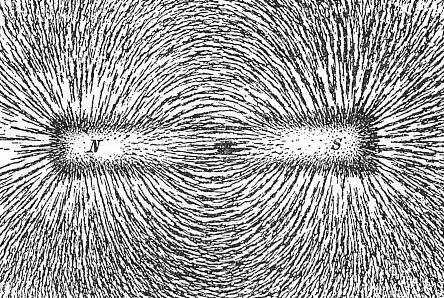
\includegraphics[width=.9\linewidth]{../figs/Magnet0873.png}
\end{center}
\end{frame}

\begin{frame}[label={sec:orgfb743b8}]{Ley de Oersted y Biot-Savart}
\begin{itemize}
\item Una corriente eléctrica crea un campo magnético en torno al
conductor.
\end{itemize}

\begin{center}
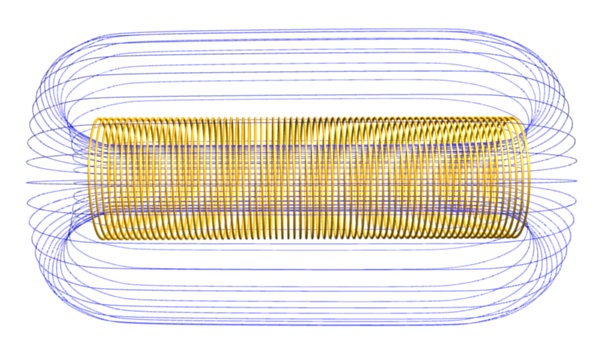
\includegraphics[width=.9\linewidth]{../figs/Solenoide.jpg}
\end{center}
\end{frame}

\begin{frame}[label={sec:org4cc61ff}]{Fuerza de Ampere}
\begin{itemize}
\item Un conductor por el que circula corriente, situado en el seno de un
campo magnético, altera este campo magnético, y experimenta una
fuerza que lo expulsa para disminuir la alteración.
\end{itemize}

\begin{center}
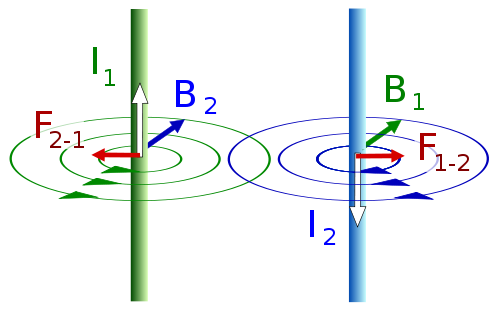
\includegraphics[width=.9\linewidth]{../figs/FuerzasRepulsion.png}
\end{center}

\begin{center}
Vídeo: \href{http://www.youtube.com/watch?v=2j8D\_N1v0tU}{Repulsión entre barras de Alta Tensión}
\end{center}
\end{frame}

\begin{frame}[label={sec:orgb3be910}]{Flujo Magnético}
El flujo magnético es la cantidad de líneas de fuerza magnética que atraviesan una superficie. Depende de la densidad de campo, \(B\), el área de la superficie, \(A\), y la posición relativa entre ambos, \(\theta\).

\[
\phi = B \cdot A \cdot \cos \theta
\]

\begin{center}
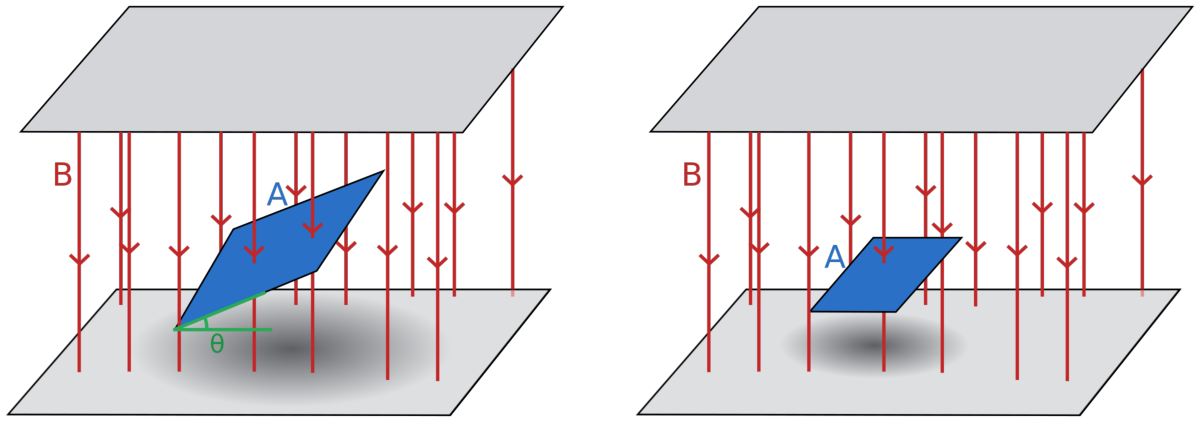
\includegraphics[width=.9\linewidth]{../figs/flujo_magnetico.pdf}
\end{center}
\end{frame}

\begin{frame}[label={sec:orgc9a4662}]{Ley de Faraday}
\begin{itemize}
\item Cuando el \alert{flujo magnético} que atraviesa una espira es \alert{variable}
aparece \alert{tensión inducida}.
\end{itemize}

\[
e=-\frac{\mathrm{d}\phi}{\mathrm{d}t} = -\frac{\mathrm{d}(B \cdot S\cdot \cos \theta)}{\mathrm{d}t} 
\]

\begin{itemize}
\item El flujo es variable cuando:

\begin{itemize}
\item La \alert{espira está en movimiento} (\(\theta\))

\item El \alert{campo magnético \(B\) es variable},

\item Ambas situaciones coinciden.
\end{itemize}

\item La tensión inducida es directamente proporcional a la rapidez de la
variación.
\end{itemize}
\end{frame}


\begin{frame}[label={sec:org5366ea5}]{Inductor e Inducido}
\begin{itemize}
\item Al elemento que emite el campo magnético se le denomina \alert{inductor} y
aquel que es atravesado por este flujo es el \alert{inducido}.
\end{itemize}
\begin{center}
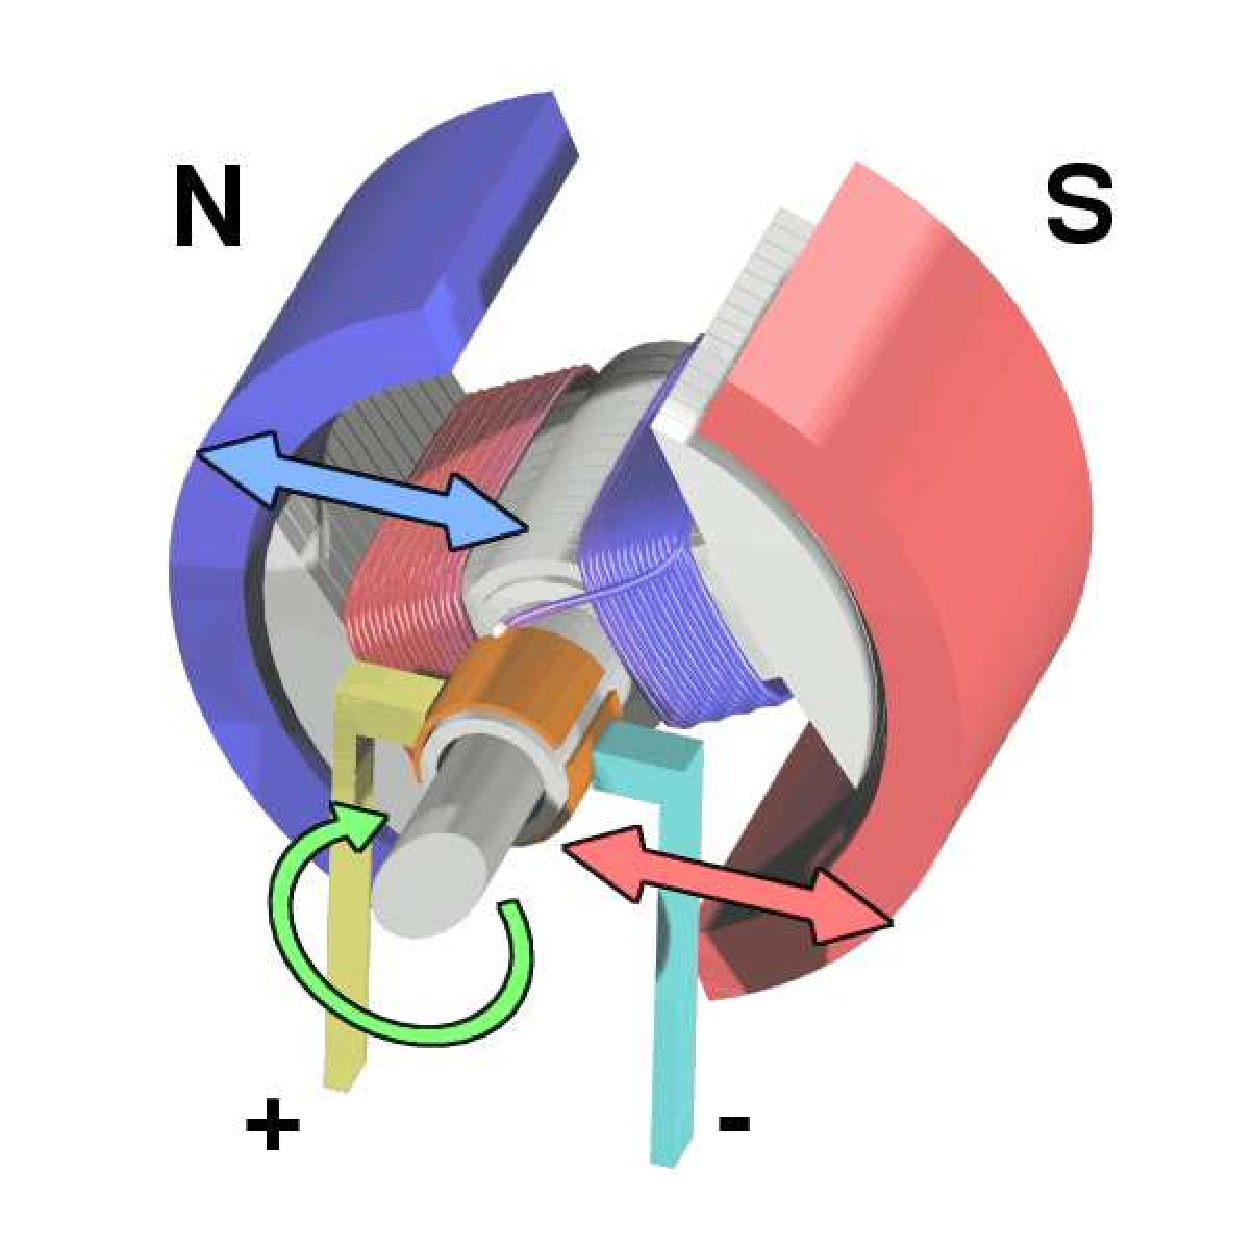
\includegraphics[height=0.7\textheight]{../figs/Electric_motor_cycle_3.pdf}
\end{center}
\end{frame}

\begin{frame}[label={sec:org6958dfd}]{Par, potencia y velocidad}
\[
  P =  T \cdot \omega
\]


\begin{itemize}
\item \(P\) es potencia mecánica; \(T\) par mecánico; \(\omega\) es la velocidad
angular.

\item El par busca alinear los ejes magnéticos de inductor e inducido, o de
estator y rotor. Una vez que están alineados, el par es nulo.
\end{itemize}
\end{frame}

\section{Máquinas Eléctricas}
\label{sec:orgcb4d82e}


\subsection{Tipos de máquinas}
\label{sec:orgf2fd9b6}


\begin{frame}[label={sec:org253be6d}]{Relación de Frecuencias}
\begin{block}{Frecuencia eléctrica y velocidad}
\(\begin{aligned}
  f_{2} & = & f_{1}-n\cdot p\end{aligned}\)

\begin{itemize}
\item \(f_{2}\) es la frecuencia en el inducido; \(f_{1}\) es la frecuencia en
el inductor; \(n\) es la velocidad angular; \(p\) es el número de polos.

\item Al utilizar colector de delgas (escobillas) en el inducido, la
frecuencia en el circuito exterior (\(f_{L}\)) es diferente a \(f_{2}\).
\end{itemize}
\end{block}
\end{frame}

\begin{frame}[label={sec:org314e054}]{Clasificación de máquinas}
\begin{itemize}
\item Estáticas (\(n=0\Rightarrow f_{2}=f_{1}\)): Transformadores

\item Rotativas (\(n\neq0\)):

\begin{itemize}
\item Flujo inductor constante (\(f_{1}=0\Rightarrow f_{2}=n\cdot
            p\))

\begin{itemize}
\item Delgas (\(f_{L}\neq f_{2}\)): Máquinas de corriente continua

\item Anillos (\(f_{L}=f_{2}\)): Máquinas síncronas
\end{itemize}

\item Flujo inductor variable (\(f_{1}>0\Rightarrow
            f_{2}=f_{1}-n\cdot p\))

\begin{itemize}
\item Delgas (\(f_{L}\neq f_{2}\)): Motor universal

\item Anillos (\(f_{L}=f_{2}\)): Máquinas asíncronas
\end{itemize}
\end{itemize}
\end{itemize}
\end{frame}

\begin{frame}[label={sec:orga835cca}]{Transformador}
\begin{itemize}
\item Un transformador consiste en dos bobinas acopladas magnéticamente.

\item Un transformador ideal tiene las siguientes relaciones entre tensión
y corriente de entrada (primario) y salida (secundario):
\end{itemize}

\(N_{s}\cdot I_{s}=N_{p}\cdot I_{p}\)
\(\frac{V_{p}}{N_{p}}=\frac{V_{s}}{N_{s}}\)

\begin{center}
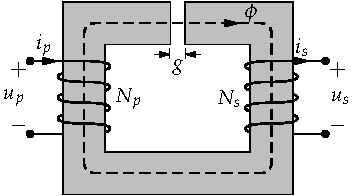
\includegraphics[height=0.3\textheight]{../figs/Transformador2.pdf}
\end{center}
\end{frame}

\begin{frame}[label={sec:orgab5b86b}]{Transformador}
\begin{itemize}
\item Un transformador ideal con relación de transformación \(N_{p}/N_{s}<1\)
(más vueltas en el secundario que en el primario), sube tensión
(\(V_{s}>V_{p}\)) y reduce corriente (\(I_{s}<I_{p}\)).
\end{itemize}

\begin{center}
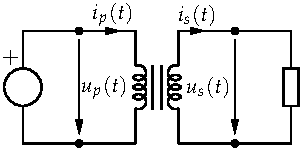
\includegraphics[width=.9\linewidth]{../figs/Transformador.pdf}
\end{center}
\end{frame}

\begin{frame}[label={sec:orgaae0a0d}]{Motores}
\begin{block}{Motor DC}
\begin{itemize}
\item \(f_{1}=0\); \(f_{L}=0\);

\item Estator-Inductor alimentado por corriente DC (o imanes permanentes).

\item El colector de delgas transforma la frecuencia de alimentación (DC)
en alterna.

\item Rotor-Inducido gira sincronizado con la frecuencia \guillemotleft{}transformada\guillemotright{}.
\end{itemize}
\end{block}
\end{frame}

\begin{frame}[label={sec:orgcd18107}]{Motores}
\begin{block}{Motor asíncrono o de inducción}
\begin{itemize}
\item \(f_{1}\neq0\);

\item Estator-inductor alimentado por una corriente trifásica alterna.
Produce un campo giratorio.

\item Rotor-inducido constituido por espiras cortocircuitadas (jaula de
ardilla).

\item Se produce un par que busca alinear el eje de las espiras con el
campo inducido. El rotor se mueve siguiendo al campo giratorio.

\item La velocidad de giro es inferior a la frecuencia de alimentación
(asíncrono).
\end{itemize}

\begin{center}
Vídeos: Motor de inducción artesanal \href{http://www.youtube.com/watch?v=ZRGlAu0uCHY\&feature=related}{(1)} \href{http://www.youtube.com/watch?v=P-eTLmJC2cQ}{(2)}
\end{center}
\end{block}
\end{frame}
\begin{frame}[label={sec:org31ec911}]{Generadores}
\begin{block}{Generador Síncrono o Alternador}
\begin{itemize}
\item \(f_{1}=0\);

\item Rotor-inductor alimentado por corriente continua mediante anillos.

\item Estator-inducido constituido por un devanado trifásico.

\item Al aplicar energía mecánica en el eje del rotor y alimentarlo con
corriente continua, se obtiene una fuerza electromotriz en el
estator.

\item Empleado en turbinas hidráulicas y térmicas.
\end{itemize}
\end{block}
\end{frame}

\begin{frame}[label={sec:org13fcbb6}]{Generadores}
\begin{block}{Dinamo}
\begin{itemize}
\item \(f_{1}=0\); \(f_{L}=0\);

\item Estator-Inductor alimentado por corriente DC (o imanes permanentes).

\item El colector de delgas transforma la frecuencia de alimentación (DC)
en alterna.

\item Al aplicar energía mecánica en el eje del rotor y alimentar el
estator con corriente continua, se obtiene una fuerza electromotriz
en el inducido con \(f_{2}\).

\item Las delgas rectifican para obtener \(f_{L}=0\) en la salida.
\end{itemize}
\end{block}
\end{frame}

\section{Aparamenta eléctrica}
\label{sec:orgb5da13c}

\subsection{Sistema de Suministro Eléctrico}
\label{sec:orgbbf1274}
\begin{frame}[label={sec:org7d97b31}]{Sistema de suministro eléctrico}
Un \alert{sistema de suministro eléctrico} tiene como objetivo \alert{producir,
transportar y distribuir energía eléctrica} a los lugares de consumo,
con el mínimo coste posible en condiciones de \alert{fiabilidad, calidad y
seguridad}.
\end{frame}

\begin{frame}[label={sec:org3e4531d}]{Componentes del Sistema de Suministro Eléctrico}
\begin{center}
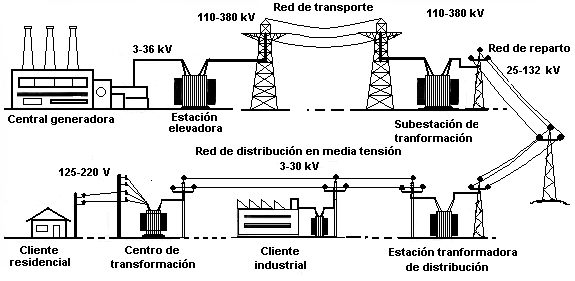
\includegraphics[width=.9\linewidth]{../figs/Redelectrica2.png}
\end{center}

\begin{itemize}
\item Generadores

\item Redes de transporte

\item Redes de distribución

\item Equipos de acondicionamiento, transformación y protección (y en
algunos casos, almacenamiento)

\item Puntos de consumo
\end{itemize}
\end{frame}


\subsection{Definición y Funciones}
\label{sec:orgac17731}
\begin{frame}[label={sec:org0a083bc}]{Definición}
\begin{block}{ITC-BT-01}
\begin{description}
\item[{Aparamenta:}] Equipo, aparato o material previsto para ser conectado a un circuito eléctrico con el fin de asegurar una o varias de las siguientes funciones: \alert{protección}, \alert{control}, \alert{seccionamiento}, \alert{conexión}.

\item[{Función de la Aparamenta:}] Garantizar la seguridad de las personas,
la continuidad en el suministro y la protección de los elemento de la
instalación.
\end{description}
\end{block}
\end{frame}

\begin{frame}[label={sec:org20ef8bd}]{Funciones de la aparamenta}
\begin{itemize}
\item \alert{Protección}:

\begin{itemize}
\item Protección de los elementos de los circuitos contra las tensiones
térmicas y mecánicas de las corrientes de cortocircuito.

\item Protección de las personas en caso de producirse un defecto de
aislamiento.

\item Protección de los dispositivos y aparatos suministrados.
\end{itemize}
\end{itemize}
\end{frame}

\begin{frame}[label={sec:org4c389f2}]{Funciones de la aparamenta}
\begin{itemize}
\item \alert{Aislamiento}: separar de forma verificable un circuito, un aparato o
un elemento de la planta del resto de un sistema que se encuentra en
tensión, con el fin de que el personal pueda realizar con total
seguridad trabajos en la parte aislada.
\end{itemize}
\end{frame}

\begin{frame}[label={sec:org83b6fb8}]{Funciones de la aparamenta}
\begin{itemize}
\item \alert{Control:} modificar un sistema cargado en cualquier momento

\begin{itemize}
\item Control funcional (conmutación rutinaria, etc.).

\item Conmutación de emergencia.

\item Operaciones de mantenimiento del sistema de alimentación.
\end{itemize}
\end{itemize}
\end{frame}

\begin{frame}[label={sec:orga83fc72}]{Arco Eléctrico}
\begin{itemize}
\item Descarga eléctrica que se forma entre dos electrodos sometidos a una diferencia de potencial.
\item Durante el tiempo de la descarga se produce una luminosidad muy intensa y un gran desprendimiento de calor.
\item Ambos fenómenos, en caso de ser accidentales, pueden ser sumamente destructivos.
\end{itemize}

\begin{center}
Vídeo: \href{http://www.youtube.com/watch?v=WBTvGqRA4\_0}{Apertura en Alta Tensión}
\end{center}
\end{frame}

\begin{frame}[label={sec:org54319ee}]{Poder de corte y cierre}
\begin{description}
\item[{Poder de corte:}] intensidad de corriente que este dispositivo es
capaz de cortar, bajo una tensión de restablecimiento determinada.

\item[{Poder de cierre:}] intensidad de corriente que este aparato es capaz
de establecer, bajo una tensión dada.
\end{description}
\end{frame}

\subsection{Tipos de Dispositivos}
\label{sec:org7eac2ea}
\begin{frame}[label={sec:org28e1a78}]{Dispositivos simples}
\begin{block}{Seccionador}
\begin{itemize}
\item Dispositivo de dos posiciones (abierto/cerrado) enclavable y accionado manualmente que proporciona un aislamiento seguro de un circuito cuando está enclavado en la posición abierta.

\item Un seccionador no está diseñado para abrir o cerrar el paso de la corriente.
\end{itemize}
\end{block}

\begin{block}{Interruptor de carga}
\begin{itemize}
\item Dispositivo no automático (accionamiento manual) de dos posiciones (abierto/cerrado).
\item Se utiliza para cerrar y abrir circuitos cargados en condiciones normales de circuitos sin defectos.
\end{itemize}
\end{block}
\end{frame}

\begin{frame}[label={sec:orgccedab7}]{Dispositivos simples}
\begin{block}{Contactor}
\begin{itemize}
\item Dispositivo accionado por solenoide que por lo general se mantiene cerrado mediante una corriente (reducida).

\item Se suelen controlar de forma remota por medio de pulsadores de activación/desactivación.
\end{itemize}
\end{block}

\begin{block}{Fusible}
\begin{itemize}
\item Un filamento o lámina de un metal o aleación de bajo punto de fusión que se intercala en un punto determinado de una instalación eléctrica

\item Se funde por Efecto Joule cuando la intensidad de corriente supere, por un cortocircuito o un exceso de carga.

\item Es capaz de abrir un circuito en carga.
\end{itemize}
\end{block}
\end{frame}

\begin{frame}[label={sec:orgdda3d02}]{Interruptor magnetotérmico}
\begin{itemize}
\item Dispositivo automático capaz de interrumpir la corriente eléctrica de un circuito cuando ésta sobrepasa ciertos valores máximos.

\item El dispositivo consta de dos partes, un electroimán y una lámina bimetálica, conectadas en serie y por las que circula la corriente que va hacia la carga.

\item Su funcionamiento se basa en dos de los efectos producidos por la circulación de corriente eléctrica en un circuito: el magnético y el térmico (efecto Joule).

\item Se emplea para \alert{proteger contra sobreintensidades y sobrecargas}.
\end{itemize}

\begin{center}
Vídeo: \href{http://www.youtube.com/watch?v=c6QqnLgWbCQ}{Apertura de un PIA}
\end{center}
\end{frame}

\begin{frame}[label={sec:orgab89f1d}]{Interruptor Magnetotérmico}
\begin{center}
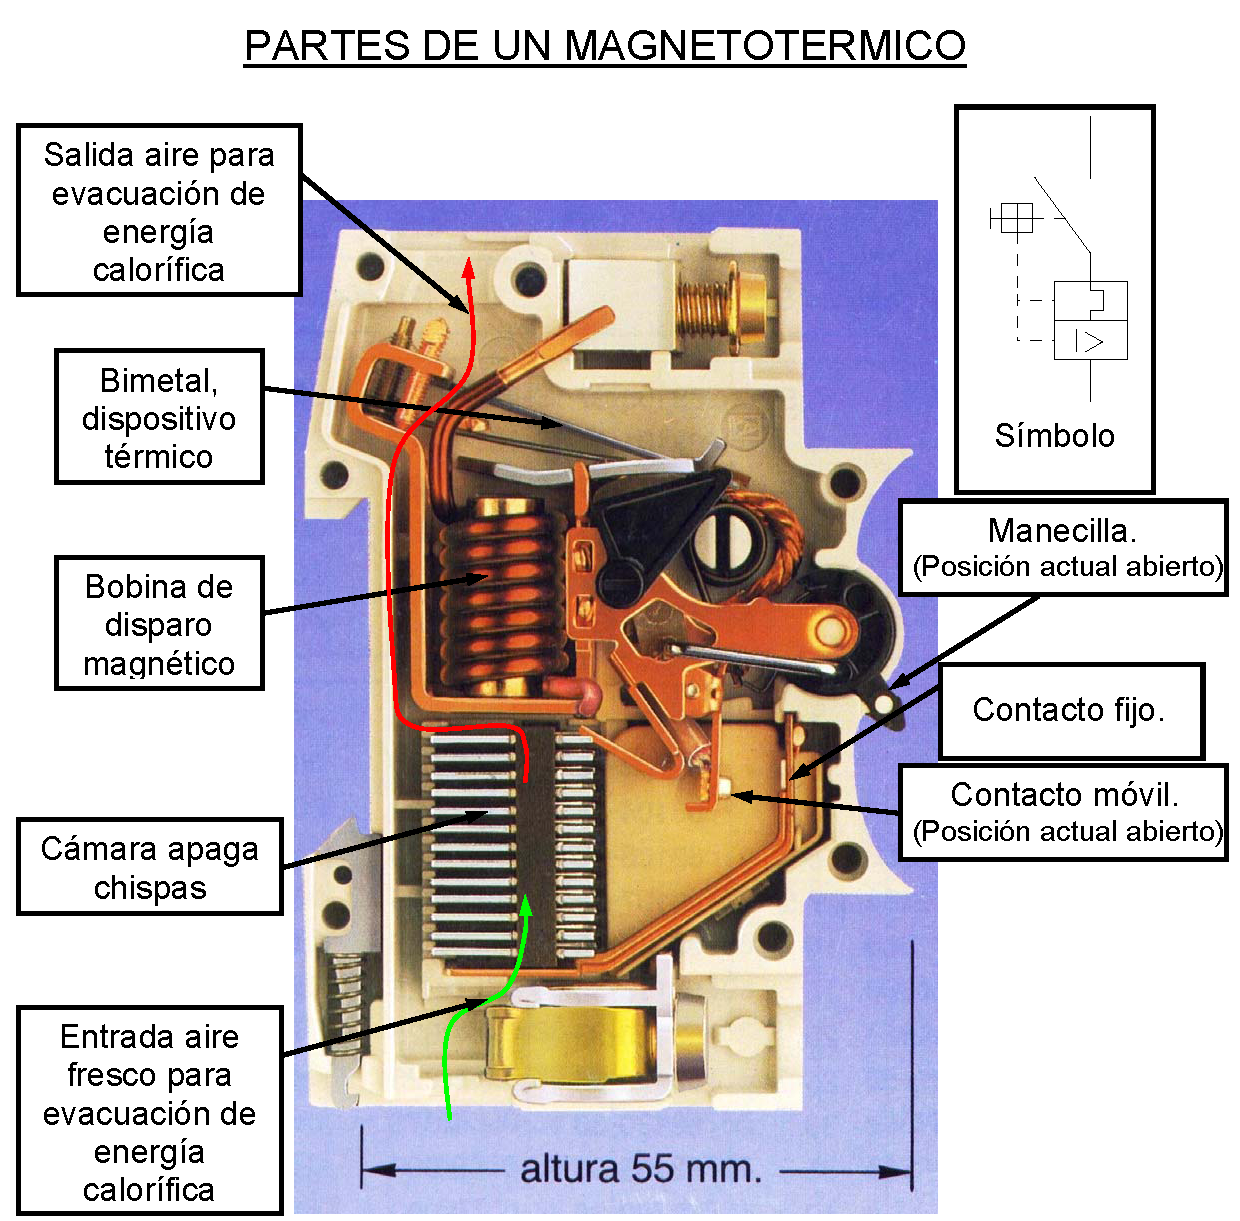
\includegraphics[height=0.8\textheight]{../figs/SeccionMagnetotermico.png}
\end{center}
\end{frame}

\begin{frame}[label={sec:org0750865}]{Interruptor diferencial}
\begin{itemize}
\item Dispositivo automático capaz de interrumpir la corriente eléctrica de un circuito cuando existe una corriente diferencial residual, indicativa de un defecto de aislamiento.
\item Para la detección emplea un transformador toroidal que abraza a todos los conductores.
\item Cuando existe un defecto, la suma fasorial de las corrientes abarcadas no será nula y, por tanto, aparecerá una intensidad en el secundario del transformador, proporcional al defecto.
\item Se emplea para la \alert{protección de las personas}.
\end{itemize}
\end{frame}

\begin{frame}[label={sec:orgc43f49a}]{Interruptor Diferencial}
\begin{center}
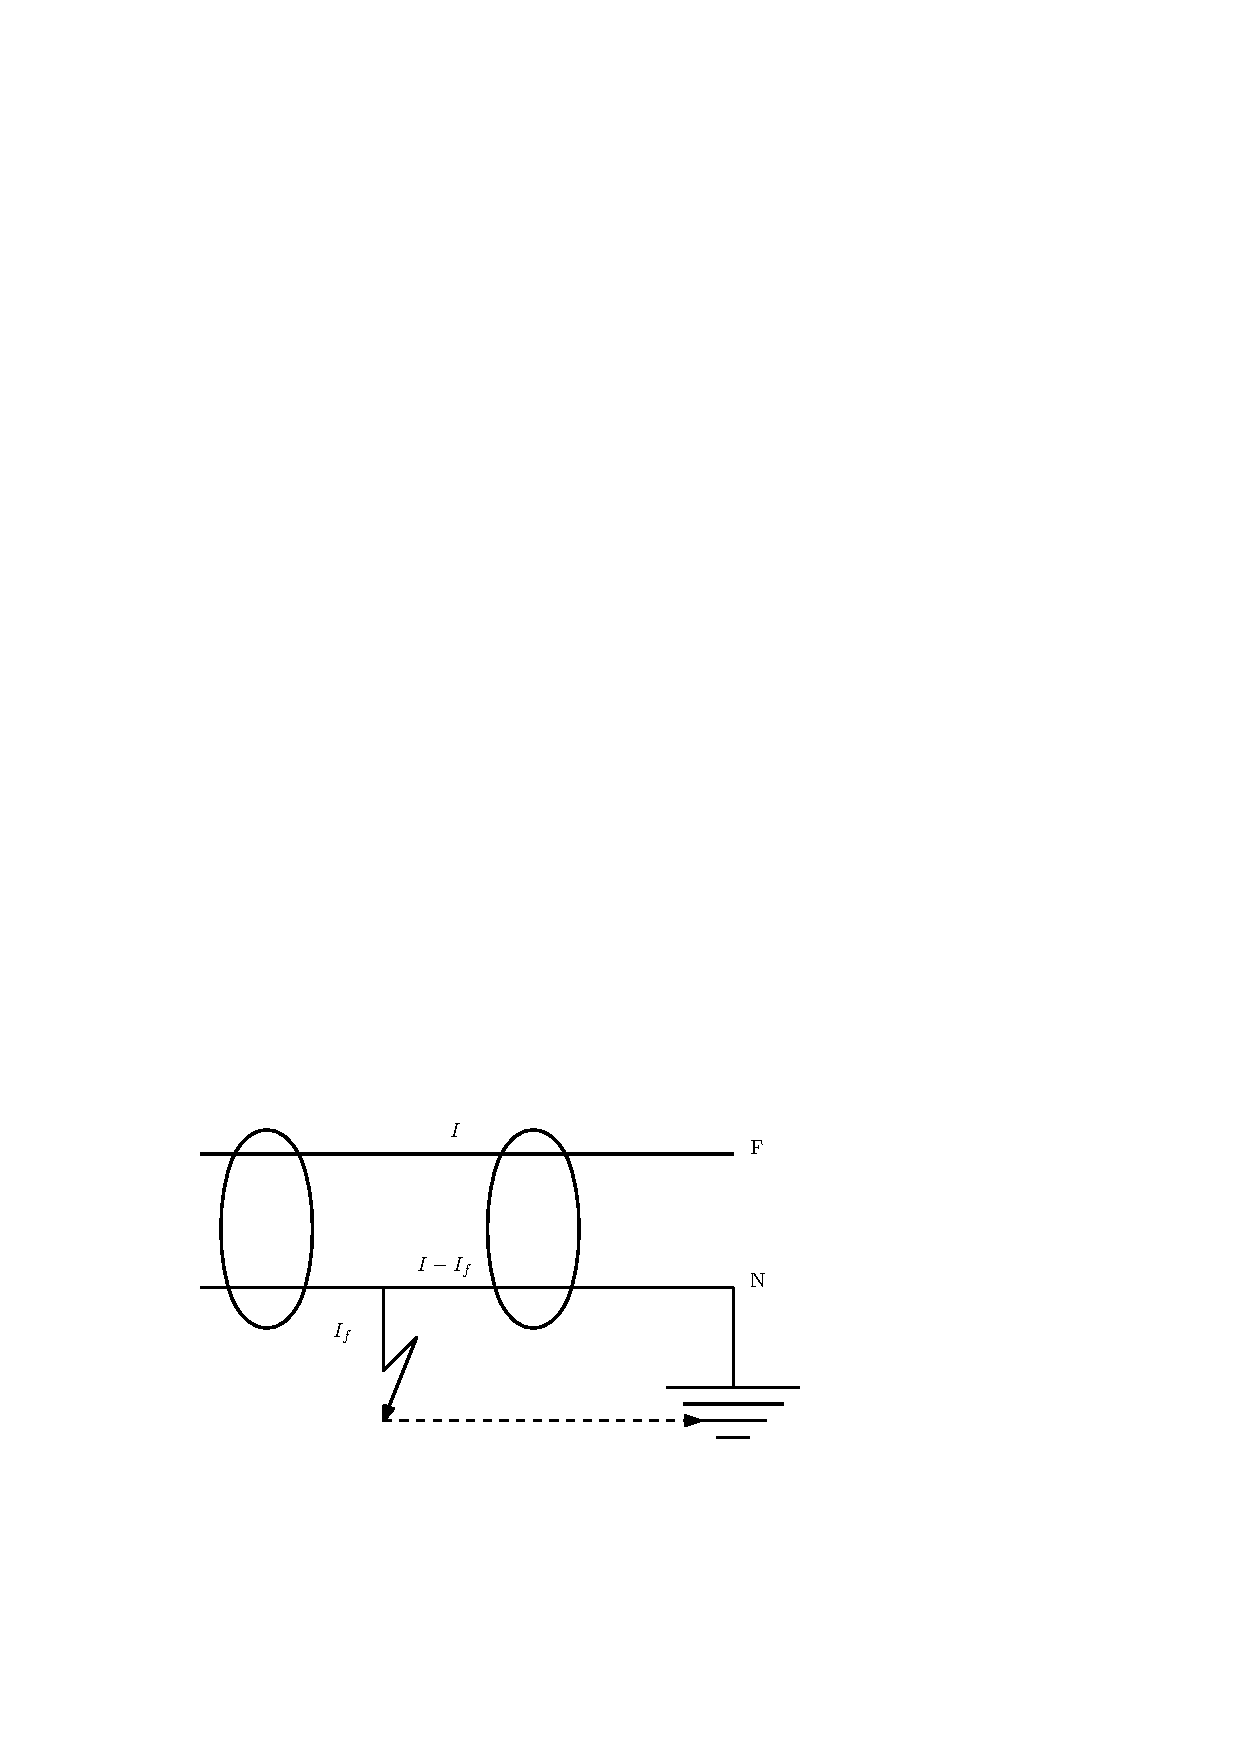
\includegraphics[height=0.3\textheight]{../figs/InterruptorDiferencial.pdf}
\end{center}

\begin{center}
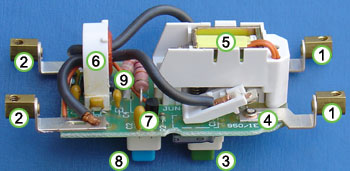
\includegraphics[height=0.3\textheight]{../figs/ResidualCurrentCircuitBreak.jpg}
\end{center}
\end{frame}

\section{Recursos}
\label{sec:org5bd192d}

\begin{itemize}
\item \alert{Fraile Mora, J.}: \emph{Máquinas Eléctricas}. Ed. Mc. Graw Hill.

\item \href{http://www.f2i2.net/legislacionseguridadindustrial/Si\_ambito.aspx?id\_am=76}{Reglamento Electrotécnico de Baja Tensión}

\item \href{https://www.schneider-electric.es/es/download/document/020511E10/}{Guía de diseño de instalaciones eléctricas (Schneider Electric)}

\item \href{http://www.directindustry.com/}{Equipos industriales}

\item \href{http://www.preoc.es/}{Base de Precios PREOC}
\end{itemize}
\end{document}